%\documentclass{acm_proc_article-sp}
\documentclass{sig-alternate}
\usepackage{amsmath}
\usepackage{amssymb}
\usepackage{listings}
\usepackage{courier}
\usepackage{multirow}

% Include PDF graphics, configure our images directory, and specify image types.
\usepackage{graphicx}
\usepackage{epsfig}
\graphicspath{{./images/}}
\DeclareGraphicsExtensions{.pdf,.jpeg,.png,.jpg}

% Style listings
\lstset{%rulesepcolor=\color{Gray},
        frame=single,                        	% Shadow box frame around code
        basicstyle=\scriptsize\ttfamily,        % Use small true type font
        showstringspaces=false,                 % Don't put marks in string spaces
        morecomment=[l][\color{Blue}]{...},     % Line continuation (...) like blue comment
}

\begin{document}

\title{Toward Quantitative Emulation of Cloud Robotic Systems}

\numberofauthors{1}

\author{
\alignauthor
Christopher C. Lamb, Rafael Figueroa, Rafael Fierro\\
       \affaddr{University of New Mexico}\\
       \affaddr{Department of Electrical and Computer Engineering}\\
       \affaddr{Albuquerque, NM 87131-0001}\\
       \email{\{cclamb, rafa, rfierro\}@unm.edu}
}

\conferenceinfo{ICCPS '14,} {April 14-17, 2014, Berlin, Germany.} 
\CopyrightYear{2014} 
\crdata{978-1-4503-1005-5/11/10} 
\clubpenalty=10000 
\widowpenalty=10000

\maketitle

\begin{abstract}
Networks of collaborating autonomous cyber-physical systems are just beginning to be able to take advantage of cloud computing.  As the advantages of using cloud computing become more obvious and validated in other fields, cloud computing will inevitably begin to migrate into autonomous system development.  Our goal overall is to begin to provide quantitative guidance around how system developers can take advantage of cloud computing within their systems.  In order to do this, we have embarked on two specific research thrusts; the first, building a cloud computing framework specifically tailored to the unique needs of autonomous systems, and the second, developing the appropriate simulation, emulation, and other tools needed to facilitate autonomous system cloud development.  Our first step, outlined within this paper, is to develop an initial taxonomy of the types of distributed system architectures system developers will likely use, to notionally describe where and when they should be used, and how they could be developed and integrated.
\end{abstract}

\category{D.2.11}{Software}{Software Architectures}[Domain-specific Architectures]
\terms{Design, Performance, Robotics}
\keywords{Robotics, Cloud}

\section{Introduction}
In the last two years, the robotics and autonomous systems community has begun looking closely at cloud computing to determine its efficacy in helping shoulder the computational load of systems.  Overall, the consensus is that cloud computing is positioned to make as large as an impact in robotics over the next few years as it has in general Information Technology in the last.  Projects that have begun to explore distributed knowledge management have demonstrated promising results~\cite{TeKlPaBe:11, TePeLaBe:12, WaBeCiDa:11}, and have spawned other similar approaches in related domains.  

We believe this approach to using cloud computing to help shoulder the computational burden for autonomous systems is not only promising, but here to stay, and also fraught with unique challenges.  First, the economic benefits seem undeniable.  Just as the cost and flexibility of cloud systems provided by commercial service providers like Amazon and Rackspace have encouraged an exodus of processing power from the company data center to the cloud, similar flexibility and cost savings will exist for robotics engineers.  Today, in order to provision a network of robots, researchers need to acquire and administer laboratory computers, networks, and robotic systems prior to making any progress.  Furthermore, these resources are centralized within a single laboratory and are usually inaccessible remotely.  This leads to the very problem cloud computing set out to solve; an high capital-intensive barrier to entry and  inconvenient resource centralization.  Incorporating cloud computing into typical experimental environments makes processing power and storage more accessible than ever before, promising to bring new engineers into robotics as the Arudino brought programmers into the world of micro-controllers.  

Not only can cloud computing lower barriers to entry, it can also more effectively provide processing power to networked autonomous systems.  Instead of requiring local data storage and processing power, or planning systems that while remote are still centralized on a single workstation in a laboratory, the ability to take advantage of the virtually unlimited computational resources of cloud computing allows robots to run just about anywhere, distributing computation allows for resoure intensive applications to be offloaded from robots to inexpensive cloud systems.

While the argument in favor of cloud computing for robotic systems mirrors that used with respect to traditional server-based computing, there are some distinct differences between the computation, storage, and communication needed by autonomous systems as opposed to simple servers or workstations.  For example, communication latencies have a much larger impact on autonomous systems than non-mobile systems.  An actuator managing a floodgate and controlled by cloud-integrated micro-controller afford to wait for direction from an external service under flood conditions.  Likewise, a cloud-enabled grasping arm needs to be able to quickly acquire grasping information from external sources whenever confronting a new object.  

This presents challenges to those conducting research into cloud robotics however.  In the past, research groups including ours has conducted experimental work using physical robotic systems mirroring those upon which we propose to execute developmental algorithms or deploy sensor platforms.  This approach will not work when conducting cloud computing research.  Researchers will not be able to afford the numbers of autonomous systems required to test approaches at realistic scale.  As a result, we feel that it is vital that the community begin to develop verified and validated simulation and emulation tools that enable researchers to easily test approaches at simulated scale.  We believe these tools must be able to run on a variety of systems, ranging from laptops for quick and dirty experimentation, to systems that incorporate physical resources like cloud nodes and robots and robotic constellations.

In order to effectively build these kinds of systems and the tools needed to emulate them, we must first understand what kinds of systems we could build, under what circumstances, and why.  

\section{Cyber-physical Clouds}
In 2012, Hu, Ta, and Wen outlined specific differences between specific types of robotic communication in clouds \cite{HuTaWe:12}.  Specifically, they rigorously described the differences between machine-to-machine and machine-to-cloud communications, and analysed optimum communication and computation distribution based on energy requirements.  A valid and useful perspective, we intend to expand this to provide practical guidance with respect to how partition computation and data storage from an implementation perspective.  We propose a structured way to look at cloud robotic systems based on the individual robot, the specific task, and the context in which the robot is executing that task.  Based on this description, we intend to establish quantitative guidance and qualitative heuristics that help system designers determine how storage, computation, and communication can be distributed and dynamically tuned in operational systems.

First, we need to clearly define what we mean by {\sl cloud robotics}.  In order to clarify this frequently overloaded term, we turn to the US National Institute for Standards and Technology (NIST), the most authoritative group to yet propose a cloud computing definition.  In Special Publication 800-145, Mell and Grance go into great detail describing clouds and different cloud types~\cite{NIST-SP-800-145}. They define cloud computing as having five {\sl essential characteristics}, three {\sl service models}, and four {\sl deployment models}.  The service models include such logical functional partitions as Software as a Service, Infrastructure as a Service, and Platforms as a Service, while deployment models include various cloud types like public, private, hybrid, and community clouds.  Service models certainly have an impact on the type of computing offered to robotic platforms, in that robots could consume exposed cloud functions in any of these service models.  Interestingly, individual systems or constellations could be offered as a PaaS or IaaS offering to interested consumers as well, implying that as robots can take advantage of cloud computation, perhaps computational systems can take advantage of constellations of robots.  In the scope of our current work however, we are most interested currently in the five essential characteristics of cloud computation:

\begin{itemize}
\item {\bf On-demand Self Service} --- Services can be easily provisioned without human intervention at a service provider.
\item {\bf Broad Network Access} --- Services are ubiquitously available via computer networks.
\item {\bf Resource Pooling} --- There is a certain level of geographic opacity to computational services, and services are pooled and dynamically reassigned according to need.
\item {\bf Rapid Elasticity} --- Services can rapidly scape up or down according to need.
\item {\bf Measured Service} --- Service providers monitor offered services in order to more effectively manage them.
\end{itemize}

These characteristics allow us to differentiate between {\sl distributed} computation and {\sl cloud} computation.  For example, a fixed amount of data storage shared between members of a constellation would be distributed, while a virtually unlimited amount of storage shared between those same members would be a cloud service.  Likewise, a Hadoop~\cite{Hadoop} implementation in which $n$ nodes are reserved for each member would be distributed, while that same implementation with variable limits imposed by demand would be a cloud system.

Having established a baseline definition of the differences between distributed and cloud computing, we can begin to outline the various ways we can assemble cloud robotic systems.

\subsection{A Taxonomy of Architectures}
Computation services can be distributed throughout a constellation of autonomous systems.  The primary services we are interested in are processing and storage.  Communication is an important secondary service as cloud and distributed service acquisition and use, of any type, depends on communication capabilities.  This gives us three service attributes we must model to understand how different configurations impact system design.  Previous work has characterized services with respect to power consumption ~\cite{HuTaWe:12}.  While vital to designing effective robotic systems, system designers will have other characteristics in mind as well, including system latency, storage and computational performance, and overall quality of service.

In the past, experimental work we have conducted with 

Hu et. al. established two communication primitives for cloud robotic systems --- machine-to-machine (m2m) and machine-to-cloud (m2c).  Using these two primitives as reusable communication components, we can assemble them into a variety of different configurations.

Outline an initial taxonomy.

\subsection{Initial Analysis of Taxonomy}
Notionally analyze the taxonomy.

\subsection{Future Work}
We have defined how we can incorporate cloud computing into constellations of robots.  In our proposed systems we have not only proposed external cloud computing services that can be used by various autonomous members of a given constellation, we have also shown how cloud computing capability can be distributed within a given constellation.  The first common perspective on cloud computing has been addressed by others from a variety of different perspectives~\cite{LoSi:13,HuWeYo:12,YiZhGa:10}, the latter perspective on constellation embedded computing services is new and purports to have skewing effects on currently accepted communication and computation models addressing cloud robotics.  At this point, we intend analyze our proposed models using Hu's power consumption effects model ~\cite{HuWeYo:12} as well as from other attributes of interest to system designers like latency and performance.

\section{Related Work}
In 2012, Kamei et. al. proposed establishing a field of {\sl Cloud Networked Robotics}.  While not directly concerned with using cloud computing in the context of autonomous systems, Kamei and colleagues present a case supporting swarms of robots with distinct functions that collaborate to effectively support individuals.  They do however describe the need to provide distributed computation and data storage services to swarms of robots enabling information sharing and coordinated planning.  Key needs they identify for distributed computing systems include providing abstractions for individual robots, so a swarm can be automatically coordinate actions toward a goal rather than requiring programming for single entities, and the ability to share different types of information freely among cooperating robots \cite{KaNiHaSa:12}.  Lorencik in 2013 outlined the state of the art in cloud systems supporting robotics deployments, outlining advantages to using cloud computing with robots in cost and performance domains, at the expense of network connection and latency dependence \cite{LoSi:13}.  In 2012, Hu outlined both two primary patterns of communication within cloud robotics as well as rigorous guidelines. based on power demands, on when they should be used and why.  He also presented communication protocols useful in both scenarios, and presented communication performance expectations.  Overall, this thorough evaluation characterizes computation based on power utilization well, but does not address other areas of concern, like urgency and result latency.  Likewise, the structural communication patterns presented are well analyzed with respect to communication performance and information distribution, but those patterns are not yet addressed from other perspectives, like urgency, or data size, nor are specific uses motivated \cite{HuWeYo:12}.  Chen proposed viewing robots as a service withing deployed constellations in 2011.  In this model, which he did implement, he developed clear interfaces to robots using web-centric technologies in which robots could be controlled as a service rather than as a specific robotic entity. The implementation follows accepted service-oriented-architecture principles well, treating each robot as a service unit with specific services published within a larger service directory.  These services can then be aggregated into specific applications within a given robotic constellation.  Chen developed and implemented the original robot as a service model, but as of yet has not provided analytical guidance on when this kind of model is appropriate, exactly why it should be used, and how it could be implemented at scale in the presence of  \cite{YiZhGa:10}.  Quintas, in 2011, outlined and implemented a hybrid system of smart room sensors and robots integrated via message-based service oriented systems.  This use of service oriented architecture (SOA) is closely related to cloud computing systems, and though it does not display the provisioning or scale of cloud computing in the outlined system, implementation of the services on top of a cloud provider's infrastructure would certainly address this gap.  Overall, the proposed sytem is both well designed and reflects common SOA services including service discovery, and demonstrates the applicability of this general class of architectures to cloud robotics.  It does not however provide any guidance with regard to when this kind of system should be used, or how it should enhance the cost or performance of integrated robotic systems outside of implementing the Trinity Scenario.

\section{Summary and Conclusions}

%\begin{figure}[!t]
%\centering
%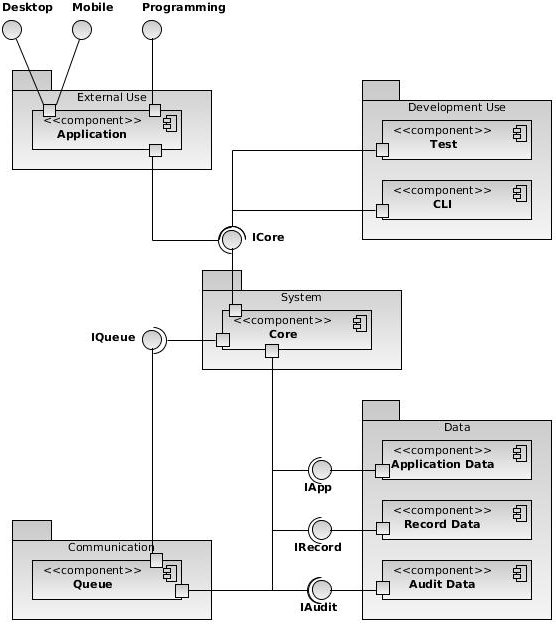
\includegraphics[width=3in]{HisbSystemArch}
%\caption{System Architecture Runtime Component View}
%\label{fig:RuntimeView}
%\end{figure}

\bibliographystyle{abbrv}
\bibliography{bib/cps.bib}

\end{document}


